\documentclass{article}
\usepackage{graphicx}
\usepackage[hidelinks]{hyperref}
\usepackage{float}
\usepackage[utf8]{inputenc}
\usepackage[spanish]{babel}
\usepackage{listings}
\usepackage[a4paper, left=3cm, right=2.5cm, top=3cm, bottom=3cm]{geometry}
\usepackage{fancyhdr}
\usepackage{lastpage}
\usepackage{minted}
\usepackage{tikz}
\usepackage{xcolor}
\usepackage[bottom]{footmisc}
\usepackage{booktabs}
\usepackage{pdflscape}
\usepackage{adjustbox}

% Definición de nuevos comandos
\newcommand{\mail}[2]{\href{mailto:#1}{#2}}
\definecolor{mygreen}{RGB}{124, 180, 76}
\definecolor{mycyan}{RGB}{100, 124, 204}

\pagestyle{fancy}
\fancyhf{}
 
\fancyfoot[R]{Página \thepage\ de \pageref{LastPage}}

% Definir un estilo para las páginas landscape con "Página X de Y" alineado a la derecha sin negrita
\fancypagestyle{landscape}{
  \fancyhf{}  % Limpiar encabezado y pie de página
  \fancyfoot{%
    \tikz[remember picture,overlay]
      \node[outer sep=2cm,above,rotate=90] at (current page.east) {Página \thepage\ de \pageref{LastPage}};}
}

\setlength{\parindent}{0pt}

\renewcommand{\headrulewidth}{0pt}
\renewcommand{\footrulewidth}{0pt}

\lstset{
    basicstyle=\ttfamily, % Estilo monoespaciado para el código
    breaklines=true,      % Romper líneas largas automáticamente
    breakatwhitespace=true, % Romper líneas largas en espacios
}

\graphicspath{{images/}}

\definecolor{highlightcolor}{rgb}{1.0, 0.76, 0.0}
\definecolor{bgcolor}{rgb}{0.95, 0.95, 0.95}

% Definición de la portada del documento
\title{
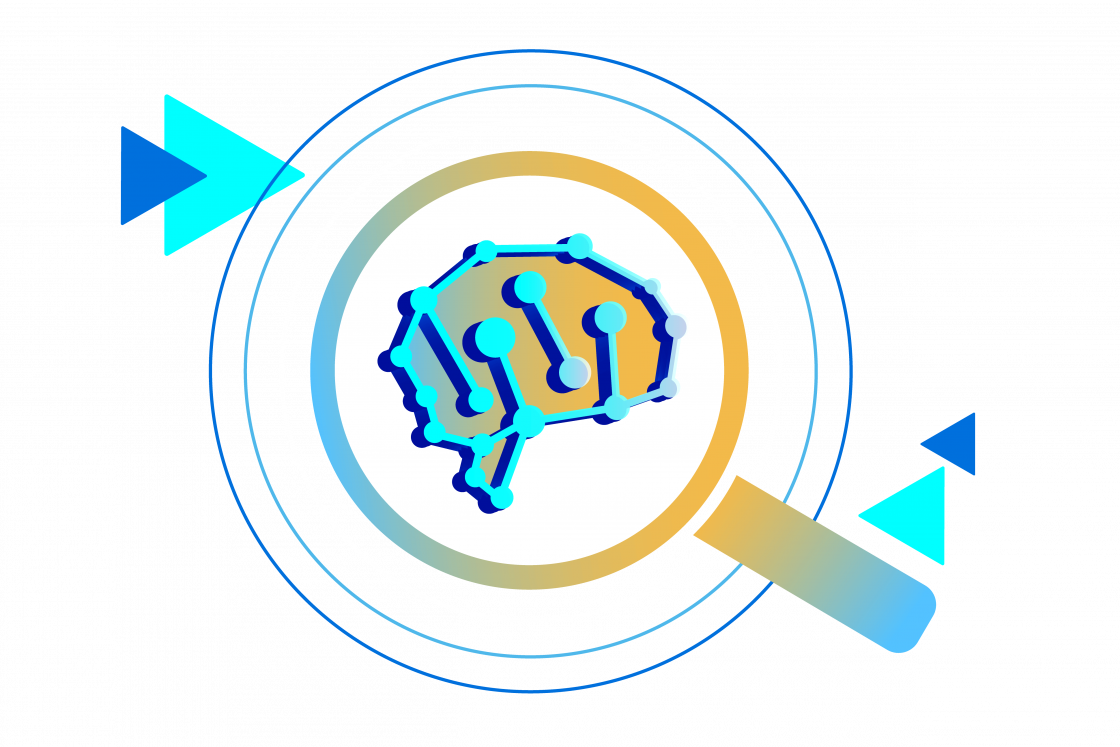
\includegraphics[scale=0.4]{deep-learning.png} \\
\vspace{2em}
\textbf{Deep Learning} \\ \rule{0.8\textwidth}{0.5pt} \\ \large \textbf{Programación de Bases de Datos}}
\author{Daniel Torres Galindo \thanks{dtorrescb@alumnos.unex.es} \and Daniel Sánchez Parra \thanks{dsanchezfe@alumnos.unex.es}}
\date{\today}

% Cambiar el formato de los números de las notas a pie de página
\makeatletter
\let\@fnsymbol\@arabic
\makeatother

\begin{document}

\maketitle

\thispagestyle{empty}

\begin{figure}[H]
    \centering
    
\includegraphics[width=0.7\textwidth]{logo-uex.png}
\end{figure}

% Línea de pie de página de la portada
\renewcommand{\footnoterule}{
    \vspace{1em}
    \hrule width \linewidth height 0.5pt
    \vspace{0.5em}
}

\newpage

\tableofcontents

\section{Introducción}
\subsection{Contexto y objetivo del proyecto}
\subsection{Justificación del uso de RNN en generación de texto}

\section{Marco Teórico}
\subsection{Introducción al Deep Learning}
\subsubsection{¿Qué es el Deep Learning?}
\subsubsection{Fundamentos del Deep Learning}
\subsubsection{Aplicaciones del Deep Learning}

\subsection{Redes Neuronales Recurrentes (RNN)}
\subsubsection{¿Qué son las RNN?}
\subsubsection{Arquitectura de las RNN}
\subsubsection{Tipos de RNN: Vanilla, LSTM, GRU, Bidireccional}
\subsubsection{Problemas de las RNN: Gradientes desvanecidos, Explosivos}

\subsection{Generación de Texto}
\subsubsection{Definición del problema}
\subsubsection{Flujo del modelo: tokenización, embeddings, RNN, decodificación}
\subsubsection{Métricas para evaluar el texto generado}

\subsection{Comparación con otros enfoques}
\subsubsection{RNN vs Transformers}

\subsection{Ventajas y Desventajas de las RNN}
\subsection{Problemas de las RNN}
\subsection{Aplicaciones de las RNN}
\subsubsection{Procesamiento del Lenguaje Natural (NLP)}
\subsubsection{Series Temporales}
\subsubsection{Reconocimiento de Voz}

\newpage

\section{Implementación Práctica}
\subsection{Preparación de Datos}
\subsubsection{Descarga y preprocesamiento del texto}
\subsubsection{Tokenización y codificación}
\subsubsection{Generación de ventanas (ventanas deslizantes)}

\subsection{Arquitectura del Modelo}
\subsubsection{Detalles de la arquitectura \texttt{CharRNN}: embeddings, LSTM, capa de salida}
\subsubsection{Hiperparámetros del modelo}
\subsubsection{Visualización de la arquitectura (diagrama opcional)}

\subsection{Entrenamiento}
\subsubsection{Configuración del entrenamiento (batch size, epochs, optimizador)}
\subsubsection{Función de pérdida y retropropagación}
\subsubsection{Monitoreo de métricas (pérdida de entrenamiento y validación)}

\subsection{Generación de Texto}
\subsubsection{Proceso de inferencia}
\subsubsection{Ajuste de la temperatura para variar la creatividad del texto generado}
\subsubsection{Ejemplos de texto generado}

\section{Resultados}
\subsection{Pérdida de entrenamiento y validación (gráficos de convergencia)}
\subsection{Ejemplos de texto generado}
\subsubsection{Texto inicial (épocas tempranas)}
\subsubsection{Texto final (épocas avanzadas)}
\subsection{Comparación con el estilo literario original (\textit{Don Quijote})}
\subsection{Observaciones sobre la coherencia del texto generado}

\newpage

\section{Conclusiones}
\subsection{Resumen de los resultados obtenidos}
\subsection{Fortalezas y limitaciones del modelo}
\subsection{Propuestas de mejora}
\subsubsection{Experimentar con GRU/LSTM más profundas}
\subsubsection{Uso de Transformers o más datos}

\section{Anexos}
\subsection{Código completo del proyecto (o enlace a un repositorio)}
\subsection{Explicación de cómo instalar y ejecutar el proyecto}
\subsubsection{Dependencias necesarias (PyTorch, tqdm, etc.)}
\subsubsection{Instrucciones para reproducir los resultados}
\subsection{Documentación adicional sobre métricas y técnicas utilizadas}

\section{Referencias}
\subsection{Artículos, libros, y recursos utilizados}
\subsubsection{Libros de Deep Learning}
\subsubsection{Documentación de PyTorch}
\subsubsection{Material académico o de investigación relevante}

\end{document}